\documentclass[12pt,a4paper]{article}

% Packages for including images, formulas, graphs, and tables
\usepackage{graphicx}
\usepackage{tikz}
\usetikzlibrary{arrows, positioning, shapes, fit, backgrounds}
\usepackage{amsmath, amssymb}
\usepackage{geometry}
\usepackage{fancyhdr}
\usepackage{titlesec}
\usepackage{hyperref}
\usepackage{setspace}
\usepackage{etoolbox} % For patching section command
\usepackage{subcaption}   % For subfigures
\usepackage{placeins}
\usepackage{longtable}   % For long tables that span multiple pages
\usepackage{booktabs}    % For professional-looking tables
\usepackage{array}       % For advanced table formatting
\usepackage{tabularx}    % For tables with adjustable column widths

% Additional packages
\usepackage{color}
\usepackage{amsfonts}
\usepackage{appendix}    % For appendix formatting

% Set page margins
\geometry{
  left=25mm,
  right=25mm,
  top=25mm,
  bottom=25mm,
}

% Set up header and footer without horizontal lines
\pagestyle{fancy}
\fancyhf{}
\cfoot{\thepage}  % Page number at the center of the footer
\renewcommand{\headrulewidth}{0pt}  % Remove header line
\renewcommand{\footrulewidth}{0pt}  % Remove footer line

% Line spacing
\onehalfspacing

% Customize section titles without lines but with numbering
\titleformat{\section}{
  \normalfont\Large\bfseries
}{\thesection.}{0.5em}{\centering}

% Customize unnumbered section titles (e.g., References) without horizontal lines
\titleformat{name=\section,numberless}
  {\normalfont\Large\bfseries}{ }{0pt}{\centering}

% Remove horizontal lines from subsections and indent with numbering
\titleformat{\subsection}{\normalfont\large\bfseries}{\thesubsection}{0.5em}{\hspace{\parindent}}

% Adjust spacing after titles
\titlespacing*{\section}{0pt}{3.5ex plus 1ex minus .2ex}{2.3ex plus .2ex}
\titlespacing*{\subsection}{0pt}{3.25ex plus 1ex minus .2ex}{1.5ex plus .2ex}

% Format \paragraph for highlighting key terms, not as a sub-subsection
\titleformat{\paragraph}
{\normalfont\normalsize\bfseries}{}{0pt}{}
\titlespacing*{\paragraph}{0pt}{1.5ex plus 1ex minus .2ex}{1em} % Adjust spacing for paragraph

% Define \textittt as \texttt for monospaced font (standard for code/filenames)
\newcommand{\textittt}[1]{\texttt{#1}}

\begin{document}

% Cover Page
\begin{titlepage}
  \centering
  \vspace*{8cm}
  {\Huge \textbf{LSE Data Analytics}}\\[1.5cm]
  {\Large \textbf{Module 1 : Data Analytics for Business}}\\[0.3cm]
  {\Large \textbf{Assignment 1 : Exploratory Data Analysis}}\\[1cm]
  {\large \today}\\[1cm]
  \begin{tabular}{ll}
    \textbf{Name:} & Alberto Berni \\
    \textbf{Email:} & \href{mailto:totoberni@gmail.com}{totoberni@gmail.com} \\
  \end{tabular}
  \vfill
\end{titlepage}

% Table of Contents
\tableofcontents
\newpage

% Start numbering pages from here (first section onwards)
\pagenumbering{arabic}
\setcounter{page}{1}

\section{The 2Market Scenario}

2Market is a retail company with a customer base across multiple countries. The company collects extensive data on customer demographics as shown by \textittt{marketing\_data.csv}, \textittt{ad\_data.csv}, and \textittt{metadata\_2Market.txt}. The analysis aims to identify customer profiles by region, determine which advertising channels are most effective, and discover product preferences across different demographic segments. This information will help 2Market optimize its marketing strategy, tailor product offerings to specific segments, and improve business performance through data-driven decision-making.
\section{Analytical Approach - PostgreSQL}
\begin{figure}[h!]
\centering
\resizebox{!}{0.15\textwidth}{
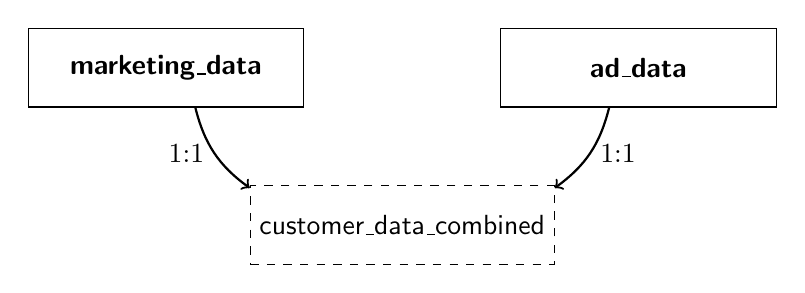
\begin{tikzpicture}[
    entity/.style={rectangle, draw, minimum width=3.5cm, minimum height=1cm, text centered, font=\sffamily\bfseries},
    pipo/.style={rectangle, draw, dashed, minimum width=3.5cm, minimum height=1cm, text centered, font=\sffamily},
    relationship/.style={diamond, draw, minimum width=2cm, minimum height=1cm, text centered, font=\sffamily\small}
]

% Initial tables
\node[entity] (marketing) at (-3,0) {marketing\_data};
\node[entity] (ad) at (3,0) {ad\_data};

% Combined table - reduced vertical space
\node[pipo] (combined) at (0,-2) {customer\_data\_combined};

% Bent arrows with relationships
\draw[->, thick] (marketing) to[bend right=20] node[midway, left] {1:1} (combined);
\draw[->, thick] (ad) to[bend left=20] node[midway, right] {1:1} (combined);

\end{tikzpicture}
}
\caption{Initial Database Schema Showing Data Integration. The 1:1 relationships represent direct mapping of records between source and combined tables.}
\label{fig:initial-schema}
\end{figure}
\noindent This analysis leverages PostgreSQL to handle structured relational data. The database is constructed in three phases: first, \textittt{tableMaking.sql} creates the correctly formatted tables for \textittt{ad\_data} and \textittt{market\_data}; next, file contents are imported through the \textittt{PgAdmin4} GUI and cleaned by \textittt{tableDataCleaning.sql} to form the unified table \textittt{customer\_data\_combined} shown in Fig.~\ref{fig:initial-schema}. Finally, three SQL scripts build views to examine the following relationships:
\paragraph{\textittt{customerDemographics.sql}}
{\footnotesize
\begin{itemize}
    \item How do customer profiles and spending behaviors vary by geographic region?
    \item Which countries show exceptional spending patterns compared to global averages?
    \item How do demographic factors (age, family size, income) differ across regions?
    \item Which marketing channels demonstrate the highest effectiveness in each country?
    \item What are the regional patterns in campaign responsiveness and complaint rates?
\end{itemize}
}
\paragraph{\textittt{adChannelAnalyis.sql}}
{\footnotesize
\begin{itemize}
    \item Which advertising channels have highest conversion rates across customer base?
    \item How do purchasing patterns and preferences differ across marketing channels?
    \item Which channels generate the highest revenue per customer?
    \item Are there any behavioral differences among customers from different channels?
    \item How do conversion patterns correlate with customer value across channels?
\end{itemize}
}
{\footnotesize
\paragraph{\textittt{productDemographics.sql}}
\begin{itemize}
    \item How do product preferences and spending vary across demographic segments?
    \item What is the relationship between age and spending power for luxury items?
    \item How does family structure influence spending and marketing responsiveness?
    \item What is the income elasticity of different product categories?
    \item How do education level and customer tenure correlate with behavioral patterns?
    \item Which demographic segments show the highest potential for targeted marketing?
\end{itemize}
}
\noindent Tabular results from these operations are reported in Sections \ref{a1:s1} - \ref{a1:s3} of the Appendix.

\subsection{Customer Demographics Analysis}
\begin{figure}[!htbp]
\centering
\resizebox{!}{!}{
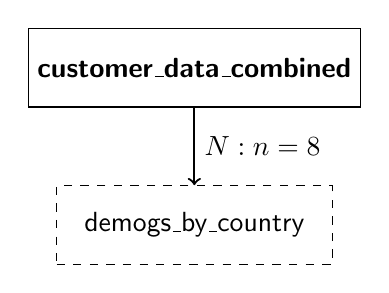
\begin{tikzpicture}[
    entity/.style={rectangle, draw, minimum width=3.5cm, minimum height=1cm, text centered, font=\sffamily\bfseries},
    pipo/.style={rectangle, draw, dashed, minimum width=3.5cm, minimum height=1cm, text centered, font=\sffamily},
    relationship/.style={diamond, draw, minimum width=2cm, minimum height=1cm, text centered, font=\sffamily\small}
]
% Primary entity
\node[entity] (combined) at (0,0) {customer\_data\_combined};
% Demographics view
\node[pipo] (demogs) at (0,-2) {demogs\_by\_country};
% Relationship
\draw[->, thick] (combined) -- (demogs) node[midway, right] {$N:n=8$};
\end{tikzpicture}
}
\caption{Customer Demographics Analysis Schema. $N:n=8$ represents the ratio of total unique customer IDs ($N$) to $n=8$, number of unique countries.}
\label{fig:demographics-schema}
\end{figure}
The demographic analysis shown in Fig.~\ref{fig:demographics-schema} reveals regional variations in customer preferences. Montenegro (ME) customers demonstrate high spending patterns, with average total spending of \$1,040.67 compared to the global average of \$607.08, particularly in alcoholic beverages (\$576.33 vs. global \$305.09); further, Spain (SP) dominates in campaign responsiveness with 52.85\% of all responses and 66.67\% of all complaints.\\
\\
Age demographics show minor variation in age (51-56 years) and family size averages between 2-3 members. Marketing channel effectiveness varies: Instagram performs best in Australia (8.16\%) and Spain (8.14\%), Twitter leads in Canada (9.02\%) and Germany (9.48\%), while Bulkmail yields effects in India (8.84\%) and Montenegro (33.33\%). This geographic variation highlights the importance of regionally targeted strategies rather than a one-size-fits-all marketing approach.
\subsection{Ad Channel Effectiveness Analysis}
Advertising channel analysis reveals Twitter (7.40\%) and Bulkmail (7.36\%) have the highest conversion rates, with Instagram close behind (7.31\%). Collectively, these three channels account for nearly 74\% of all conversions. Brochure marketing is the lowest for effectiveness at just 1.35\% conversion and 4.54\% of total conversions.
\begin{figure}[h!]
\centering
\resizebox{!}{!}{
\begin{tikzpicture}[
    entity/.style={rectangle, draw, minimum width=3.5cm, minimum height=1cm, text centered, font=\sffamily\bfseries},
    pipo/.style={rectangle, draw, dashed, minimum width=3.5cm, minimum height=1cm, text centered, font=\sffamily},
    relationship/.style={diamond, draw, minimum width=2cm, minimum height=1cm, text centered, font=\sffamily\small}
]

% Primary entity
\node[entity] (combined) at (0,0) {customer\_data\_combined};

% Ad channel analysis views
\node[pipo] (conv) at (-6,-2) {ad\_channel\_conversion};
\node[pipo] (prod) at (-2,-2) {ad\_channel\_product};
\node[pipo] (rev) at (2,-2) {ad\_channel\_revenue};
\node[pipo] (beh) at (6,-2) {ad\_channel\_behavior};

% Relationships
\draw[->, thick] (combined) to [bend right = 5] (conv) \node[below left] at (-4, -0.6) {$N:2$};
\draw[->, thick] (combined) to [bend right = 1] (prod) \node[below] at (-1.8, -0.6) {$N:7$};
\draw[->, thick] (combined) to [bend left  = 1] (rev) \node[below] at (1.8, -0.6) {$N:8$};
\draw[->, thick] (combined) to [bend left = 5] (beh) \node[below] at (4.5, -0.6) {$N:8$};

\end{tikzpicture}
}
\caption{Ad Channel Analysis Schema. The relationships show ratios of customer IDs ($N$) to number of rows in each analysis view: conversion ($n=2$ metrics), product ($n=7$ channels), revenue ($n=8$ channels), and behavior ($n=8$ channels).}
\label{fig:ad-channel-schema}
\end{figure}
\FloatBarrier
\noindent Product affinity analysis shows distinct purchasing patterns across channels. Instagram customers spend significantly more on alcoholic beverages (\$873.77) and meat products (\$467.90) compared to global averages (\$305.09 and \$167.00, respectively), while Bulkmail converts more budget-conscious customers. Revenue analysis confirms this; Instagram generates the highest customer value (\$1,616.43 per customer, 266\% of global average) despite reaching fewer customers than other channels. Facebook achieves similar results with \$1,484.35 per customer (244\% of global average).\\
\\
Behavioral analysis reveals Instagram and Facebook generate fewer but higher-value website visits, with visit-to-purchase conversion rates approximately 40\% higher than average. Bulkmail customers show lower in-store purchases (86\% of average) but higher response rates to campaigns (313\% of average). This analysis suggests channel-specific strategies: Instagram/Facebook for premium product marketing, Twitter for broader reach, and Bulkmail for campaign engagement and response.
\subsection{Product Demographics Analysis}
\begin{figure}[h!]
\centering
\resizebox{!}{!}{
\begin{tikzpicture}[
    entity/.style={rectangle, draw, minimum width=3.5cm, minimum height=1cm, text centered, font=\sffamily\bfseries},
    pipo/.style={rectangle, draw, dashed, minimum width=3.5cm, minimum height=1cm, text centered, font=\sffamily},
    relationship/.style={diamond, draw, minimum width=2cm, minimum height=1cm, text centered, font=\sffamily\small}
]

% Primary entity
\node[entity] (combined) at (0,0) {customer\_data\_combined};

% Product analysis views - first row
\node[pipo] (country) at (-6,-2) {product\_by\_country};
\node[pipo] (age) at (-2,-2) {product\_by\_age};
\node[pipo] (family) at (2,-2) {product\_by\_family};
\node[pipo] (income) at (6,-2) {product\_by\_income};

% Second row of views
\node[pipo] (edu) at (-6,0) {product\_by\_education};
\node[pipo] (tenure) at (6,0) {product\_by\_tenure};

% Relationships - first row
\draw[->, thick] (combined) -- (country) \node[] at (-4.5, -1.1){$N:9$};
\draw[->, thick] (combined) -- (age) \node[] at (-1.8, -1.1) {$N:7$};
\draw[->, thick] (combined) -- (family) \node[] at (1.8, -1.1) {$N:6$};
\draw[->, thick] (combined) -- (income) \node[] at (4.5, -1.1) {$N:7$};

% Relationships - second row
\draw[->, thick] (combined) to (edu) \node[top] at (-3.2,0.5) {$N:6$};
\draw[->, thick] (combined) to (tenure) \node[top] at (3.3, 0.5){$N:7$};

\end{tikzpicture}
}
\caption{Product Demographics Analysis Schema. Each relationship shows the ratio of unique customer IDs ($N$) to the number of demographic segments in each analysis: country ($n=8$), age ($n=6$), family size ($n=6$), income bracket ($n=6$), education level ($n=6$), and tenure group ($n=7$).}
\label{fig:product-demographics-schema}
\end{figure}
\FloatBarrier
\noindent Product demographics analysis reveals strong correlations between customer segments and purchasing patterns. Age-based analysis shows a clear correlation between age and spending power, with the oldest customer segment (Age\_Group\_6) spending 27\% more than the youngest (\$743.11 versus \$584.71). The most significant difference is alcoholic beverage purchases, where spending increases by 55\% from youngest to oldest groups (\$255.32 to \$396.41). Family structure also influences spending patterns, with single-person households spending nearly four times more per person (\$1,107.23) than five-person households (\$299.03). Response rates to marketing campaigns follow this pattern, with single-person households demonstrating five times higher response rates than $5+$ member households ($40.1\%$  versus 3.2\%).\\
\\
Income analysis reveals the most striking disparities, with the highest income bracket spending nearly 20 times more (\$1,425.13) than the lowest (\$72.18). Notably, luxury items show the highest elasticity—spending on alcoholic beverages (47.7 times from lowest to highest income brackets), while commodities spending increases by a factor of 4.2. It follows that education level shows a strong correlation with spending patterns and marketing receptiveness. PhD holders spend 8.3 times more (\$676.73) than those with basic education (\$81.80) and respond to marketing at 5.7 times the rate (21.0\% versus 3.7\%). Customer tenure analysis also demonstrates that the longest-tenured customers spend 68\% more (\$776.17) than newer customers (\$462.53), responding to marketing campaigns at nearly four times the rate (30.3\% versus 7.6\%).\\
\\
These findings provide clear segmentation guidance for 2Market: target high-value demographic segments (older, higher-income, higher-education, longer-tenure customers) with premium alcohol and meat products; develop separate strategies for family-oriented budget segments; and recognize that the highest marketing response rates come from single-person, higher-education, longer-tenured customer segments.
\clearpage
\newpage


% Start the appendix
\begin{appendix}
\section{Data Tables from SQL Analysis}\label{a1}

This appendix contains the detailed data tables generated from the SQL analysis scripts. These tables provide the raw data that supports the analysis presented in the main report.

\subsection{Customer Demographics Analysis}\label{a1:s1}
\label{app:customerdemographics}

Table~\ref{tab:demographics} shows the key demographic metrics by country, generated by the \textittt{customerDemographics.sql} script. This data provides insights into customer profiles, spending patterns, and marketing channel effectiveness across different geographic regions.

\begin{table}[h!]
\centering
\caption{Customer Demographics by Country}
\label{tab:demographics}
\resizebox{\textwidth}{!}{
\begin{tabular}{lrrrrrrrr}
\toprule
\textbf{Metric} & \textbf{AUS} & \textbf{CA} & \textbf{GER} & \textbf{IND} & \textbf{ME} & \textbf{SA} & \textbf{SP} & \textbf{US} \\
\midrule
Avg\_Age & 56.25 & 55.87 & 55.15 & 53.08 & 51.67 & 54.82 & 55.21 & 55.79 \\
Avg\_Family\_Size & 2.71 & 2.61 & 2.59 & 2.67 & 2.00 & 2.58 & 2.58 & 2.46 \\
Avg\_Income & 51804.29 & 53050.62 & 52951.09 & 49016.41 & 57680.33 & 54830.82 & 51564.58 & 53218.37 \\
Avg\_Purchase\_Frequency & 0.07 & 0.05 & 0.07 & 0.05 & 0.10 & 0.05 & 0.06 & 0.05 \\
Avg\_Total\_Spending & 582.15 & 629.33 & 631.02 & 529.29 & 1040.67 & 626.32 & 603.44 & 631.27 \\
Avg\_AmtLiq & 290.83 & 316.04 & 317.03 & 246.50 & 576.33 & 314.30 & 307.77 & 301.07 \\
Avg\_AmtVege & 25.10 & 28.88 & 25.69 & 25.77 & 2.67 & 26.52 & 25.88 & 28.36 \\
Avg\_AmtNonVeg & 151.89 & 172.65 & 174.76 & 161.42 & 272.33 & 173.29 & 163.23 & 188.64 \\
Avg\_AmtPes & 37.73 & 37.52 & 39.66 & 32.78 & 75.33 & 40.56 & 36.74 & 41.22 \\
Avg\_AmtChocolates & 28.09 & 28.60 & 24.15 & 21.91 & 40.67 & 26.76 & 27.57 & 26.76 \\
Avg\_AmtComm & 48.52 & 45.65 & 49.72 & 40.91 & 73.33 & 44.89 & 42.25 & 45.22 \\
Response\_Percentage & 6.61 & 11.41 & 5.11 & 3.90 & 0.60 & 15.62 & 52.85 & 3.90 \\
Complain\_Percentage & 0.00 & 9.52 & 4.76 & 4.76 & 0.00 & 14.29 & 66.67 & 0.00 \\
Total\_Ad\_Percentage & 5.14 & 13.16 & 5.75 & 5.75 & 0.15 & 13.01 & 53.10 & 3.93 \\
\bottomrule
\end{tabular}
}
\end{table}

\begin{table}[h!]
\centering
\caption{Top Three Marketing Channels by Country}
\label{tab:topchannels}
\resizebox{!}{!}{
\begin{tabular}{lp{11cm}}
\toprule
\textbf{Country} & \textbf{Top Three Channels} \\
\midrule
AUS & Instagram (8.16\%), Bulkmail (6.12\%), Facebook (4.76\%) \\
CA & Twitter (9.02\%), Instagram (7.89\%), Bulkmail (6.77\%) \\
GER & Twitter (9.48\%), Bulkmail (8.62\%), Instagram (6.90\%) \\
IND & Bulkmail (8.84\%), Twitter (6.80\%), Facebook (4.76\%) \\
ME & Bulkmail (33.33\%) \\
SA & Bulkmail (6.23\%), Instagram (6.23\%), Twitter (5.93\%) \\
SP & Instagram (8.14\%), Twitter (7.96\%), Bulkmail (7.59\%) \\
US & Bulkmail (7.48\%), Facebook (6.54\%), Twitter (5.61\%) \\
\bottomrule
\end{tabular}
}
\end{table}

\subsection{Ad Channel Effectiveness Analysis}\label{a1:s2}
\label{app:adchannelanalysis}

Tables~\ref{tab:conversionrates}-\ref{tab:channelbehavior} display the results of the ad channel effectiveness analysis generated by the \textittt{adChannelAnalysis.sql} script. These tables show conversion rates, product affinities, revenue, and customer behavior by marketing channel.
\clearpage
\newpage

\begin{table}[!htbp]
\centering
\caption{Ad Channel Conversion Rates}
\label{tab:conversionrates}
\resizebox{\textwidth}{!}{
\begin{tabular}{lrrrrrr}
\toprule
\textbf{Metric} & \textbf{Bulkmail} & \textbf{Twitter} & \textbf{Instagram} & \textbf{Facebook} & \textbf{Brochure} & \textbf{All Channels} \\
\midrule
Global\_Conversion\_Rates & 7.36 & 7.40 & 7.31 & 6.41 & 1.35 & 29.83 \\
Channel\_Share\_of\_Conversions & 24.66 & 24.81 & 24.51 & 21.48 & 4.54 & 100.00 \\
\bottomrule
\end{tabular}
}

\end{table}
\begin{table}[!htbp]
\centering
\caption{Product Affinities by Ad Channel}
\label{tab:productaffinities}
\resizebox{\textwidth}{!}{
\begin{tabular}{lrrrrrrl}
\toprule
\textbf{Channel} & \textbf{Alcohol} & \textbf{Vege} & \textbf{Meat} & \textbf{Fish} & \textbf{Choc} & \textbf{Comm} & \textbf{Top Three Products} \\
\midrule
All Customers & 305.09 & 26.36 & 167.00 & 37.64 & 27.03 & 43.97 & Alcohol (\$305.09), Meat (\$167.00), Commodities (\$43.97) \\
No Channel & 224.94 & 23.75 & 135.60 & 33.12 & 23.66 & 38.87 & Alcohol (\$224.94), Meat (\$135.60), Commodities (\$38.87) \\
Brochure & 898.67 & 22.97 & 250.30 & 38.73 & 30.60 & 66.40 & Alcohol (\$898.67), Meat (\$250.30), Commodities (\$66.40) \\
Bulkmail & 378.66 & 28.39 & 181.67 & 37.60 & 27.29 & 66.94 & Alcohol (\$378.66), Meat (\$181.67), Commodities (\$66.94) \\
Facebook & 758.03 & 55.52 & 435.29 & 92.37 & 65.49 & 77.65 & Alcohol (\$758.03), Meat (\$435.29), Fish (\$92.37) \\
Instagram & 873.77 & 56.51 & 467.90 & 75.90 & 64.93 & 77.43 & Alcohol (\$873.77), Meat (\$467.90), Commodities (\$77.43) \\
Twitter & 750.23 & 27.26 & 239.66 & 40.76 & 31.29 & 48.37 & Alcohol (\$750.23), Meat (\$239.66), Commodities (\$48.37) \\
\bottomrule
\end{tabular}
}
\end{table}
\begin{table}[!htbp]
\centering
\caption{Revenue Analysis by Ad Channel}
\label{tab:channelrevenue}
\resizebox{\textwidth}{!}{
\begin{tabular}{lrrrrr}
\toprule
\textbf{Channel} & \textbf{Total Revenue} & \textbf{Avg Revenue/Customer} & \textbf{Customer Count} & \textbf{\% of Total Revenue} & \textbf{\% of Avg Revenue} \\
\midrule
All Customers & 1,345,279 & 607.08 & 2,216 & 100.00 & 100.00 \\
All Ad Channels & 502,022 & 1,093.73 & 459 & 37.32 & 180.16 \\
No Channel & 843,257 & 479.94 & 1,757 & 62.68 & 79.06 \\
Instagram & 261,862 & 1,616.43 & 162 & 19.47 & 266.26 \\
Facebook & 210,777 & 1,484.35 & 142 & 15.67 & 244.51 \\
Twitter & 186,560 & 1,137.56 & 164 & 13.87 & 187.38 \\
Bulkmail & 117,448 & 720.54 & 163 & 8.73 & 118.69 \\
Brochure & 39,230 & 1,307.67 & 30 & 2.92 & 215.40 \\
\bottomrule
\end{tabular}
}
\end{table}



\begin{table}[!htbp]
\centering
\caption{Customer Behavior Analysis by Ad Channel}
\label{tab}
\resizebox{\textwidth}{!}{
\begin{tabular}{@{}lrrrrrrrrr@{}}
\toprule
\textbf{Channel} & \textbf{Purchase} & \textbf{Website} & \textbf{Web} & \textbf{Deals} & \textbf{Response} & \textbf{In-Store} & \textbf{Complaint} & \textbf{Customer} \\
& \textbf{Frequency} & \textbf{Visits} & \textbf{Buys} & & \textbf{Rate} & \textbf{Purchases} & \textbf{Rate} & \textbf{Count} \\
\midrule
All Customers & 0.0550 & 5.32 & 4.09 & 2.32 & 0.15 & 5.80 & 0.01 & 2,216 \\
All Ad Channels & 0.0552 & 4.71 & 5.22 & 1.99 & 0.41 & 6.99 & 0.00 & 459 \\
No Channel & 0.0550 & 5.48 & 3.79 & 2.41 & 0.08 & 5.49 & 0.01 & 1,757 \\
Facebook & 0.0801 & 3.51 & 5.75 & 1.39 & 0.56 & 8.02 & 0.00 & 142 \\
Brochure & 0.0720 & 5.17 & 4.90 & 1.70 & 0.67 & 8.17 & 0.00 & 30 \\
Instagram & 0.0547 & 2.92 & 5.46 & 1.06 & 0.56 & 8.27 & 0.01 & 162 \\
Twitter & 0.0524 & 5.07 & 5.66 & 2.43 & 0.38 & 7.85 & 0.00 & 164 \\
Bulkmail & 0.0482 & 5.85 & 4.50 & 2.17 & 0.47 & 5.01 & 0.01 & 163 \\
\bottomrule
\end{tabular}
}
\end{table}

\subsection{Product Demographics Analysis}\label{a1:s3}
\label{app:productdemographics}

Tables~\ref{tab:product-country}-\ref{tab:product-tenure} present the product spending and customer behavior patterns by demographic segment, generated by the \textittt{productDemographics.sql} script.

\begin{table}[h!]
\centering
\caption{Product Analysis by Country}
\label{tab:product-country}
\resizebox{\textwidth}{!}{
\begin{tabular}{lrrrrrrrrr}
\toprule
\textbf{Metric} & \textbf{Global} & \textbf{AUS} & \textbf{CA} & \textbf{GER} & \textbf{IND} & \textbf{ME} & \textbf{SA} & \textbf{SP} & \textbf{US} \\
\midrule
Total Spending & 607.08 & 582.15 & 629.33 & 631.02 & 529.29 & 1040.67 & 626.32 & 603.44 & 631.27 \\
Alcohol & 305.09 & 290.83 & 316.04 & 317.03 & 246.50 & 576.33 & 314.30 & 307.77 & 301.07 \\
Meat & 167.00 & 151.89 & 172.65 & 174.76 & 161.42 & 272.33 & 173.29 & 163.23 & 188.64 \\
Commodities & 43.97 & 48.52 & 45.65 & 49.72 & 40.91 & 73.33 & 44.89 & 42.25 & 45.22 \\
Fish & 37.64 & 37.73 & 37.52 & 39.66 & 32.78 & 75.33 & 40.56 & 36.74 & 41.22 \\
Chocolates & 27.03 & 28.09 & 28.60 & 24.15 & 21.91 & 40.67 & 26.76 & 27.57 & 26.76 \\
Purchase Frequency & 0.0670 & 0.0716 & 0.0686 & 0.0865 & 0.0789 & 0.0997 & 0.0489 & 0.0670 & 0.0744 \\
Complaint Rate & 0.0095 & 0.0000 & 0.0075 & 0.0086 & 0.0068 & 0.0000 & 0.0089 & 0.0128 & 0.0000 \\
Response Rate & 0.1503 & 0.1497 & 0.1429 & 0.1466 & 0.0884 & 0.6667 & 0.1543 & 0.1610 & 0.1215 \\
\bottomrule
\end{tabular}
}
\end{table}

\begin{table}[h!]
\centering
\caption{Product Analysis by Age Group}
\label{tab:product-age}
\resizebox{!}{0.15\textwidth}{
\begin{tabular}{lrrrrrrr}
\toprule
\textbf{Metric} & \textbf{Global} & \textbf{Age 1} & \textbf{Age 2} & \textbf{Age 3} & \textbf{Age 4} & \textbf{Age 5} & \textbf{Age 6} \\
\midrule
Total Spending & 607.08 & 584.71 & 496.05 & 521.90 & 612.98 & 684.07 & 743.11 \\
Alcohol & 305.09 & 255.32 & 235.13 & 265.35 & 320.64 & 358.03 & 396.41 \\
Meat & 167.00 & 189.42 & 137.88 & 143.15 & 158.40 & 178.17 & 194.98 \\
Commodities & 43.97 & 42.64 & 40.88 & 35.66 & 45.28 & 47.86 & 51.49 \\
Fish & 37.64 & 39.75 & 34.31 & 30.60 & 35.02 & 42.20 & 43.93 \\
Chocolates & 27.03 & 28.54 & 24.55 & 24.82 & 26.41 & 28.07 & 29.78 \\
Purchase Frequency & 0.0670 & 0.0648 & 0.0581 & 0.0650 & 0.0694 & 0.0803 & 0.0642 \\
Complaint Rate & 0.0095 & 0.0135 & 0.0135 & 0.0000 & 0.0000 & 0.0108 & 0.0190 \\
Response Rate & 0.1503 & 0.2027 & 0.1108 & 0.1545 & 0.1436 & 0.1301 & 0.1599 \\
\bottomrule
\end{tabular}
}
\end{table}

\begin{table}[h!]
\centering
\caption{Product Analysis by Family Size}
\label{tab:product-family}
\resizebox{!}{0.15\textwidth}{
\begin{tabular}{lrrrrrr}
\toprule
\textbf{Metric} & \textbf{Global} & \textbf{Size 1} & \textbf{Size 2} & \textbf{Size 3} & \textbf{Size 4} & \textbf{Size 5} \\
\midrule
Total Spending & 607.08 & 1107.23 & 785.09 & 442.96 & 246.16 & 299.03 \\
Alcohol & 305.09 & 491.20 & 375.17 & 248.84 & 145.80 & 198.94 \\
Meat & 167.00 & 371.31 & 232.28 & 95.17 & 50.49 & 63.48 \\
Commodities & 43.97 & 64.42 & 52.47 & 38.76 & 22.84 & 19.52 \\
Fish & 37.64 & 74.33 & 52.85 & 24.22 & 10.62 & 6.90 \\
Chocolates & 27.03 & 53.67 & 36.13 & 18.61 & 8.51 & 3.90 \\
Purchase Frequency & 0.0670 & 0.0543 & 0.0583 & 0.0569 & 0.0413 & 0.0574 \\
Complaint Rate & 0.0095 & 0.0040 & 0.0079 & 0.0125 & 0.0068 & 0.0323 \\
Response Rate & 0.1503 & 0.4008 & 0.1532 & 0.1034 & 0.0811 & 0.0323 \\
\bottomrule
\end{tabular}
}
\end{table}

\begin{table}[!htbp]
\centering
\caption{Product Analysis by Income Bracket}
\label{tab:product-income}
\resizebox{!}{0.15\textwidth}{
\begin{tabular}{lrrrrrrr}
\toprule
\textbf{Metric} & \textbf{Global} & \textbf{Inc 1} & \textbf{Inc 2} & \textbf{Inc 3} & \textbf{Inc 4} & \textbf{Inc 5} & \textbf{Inc 6} \\
\midrule
Total Spending & 607.08 & 72.18 & 117.42 & 280.62 & 638.26 & 1111.61 & 1425.13 \\
Alcohol & 305.09 & 13.78 & 46.87 & 159.50 & 378.86 & 575.27 & 657.75 \\
Meat & 167.00 & 21.46 & 29.73 & 55.25 & 123.63 & 298.58 & 474.09 \\
Commodities & 43.97 & 16.99 & 18.48 & 32.05 & 55.61 & 69.86 & 70.93 \\
Fish & 37.64 & 8.01 & 10.15 & 15.26 & 32.04 & 68.99 & 91.53 \\
Chocolates & 27.03 & 6.19 & 5.94 & 9.57 & 23.41 & 49.80 & 67.37 \\
Purchase Frequency & 0.0550 & 0.0536 & 0.0576 & 0.0501 & 0.0455 & 0.0650 & 0.0582 \\
Complaint Rate & 0.0095 & 0.0108 & 0.0216 & 0.0054 & 0.0054 & 0.0081 & 0.0054 \\
Response Rate & 0.1503 & 0.1054 & 0.1243 & 0.1138 & 0.0921 & 0.1436 & 0.3225 \\
\bottomrule
\end{tabular}
}
\end{table}
\clearpage
\newpage

\begin{table}[!htbp]
\centering
\caption{Product Analysis by Education Level}
\label{tab:product-education}
\resizebox{!}{0.15\textwidth}{
\begin{tabular}{lrrrrrr}
\toprule
\textbf{Metric} & \textbf{Global} & \textbf{Basic} & \textbf{2n Cycle} & \textbf{Graduation} & \textbf{Master} & \textbf{PhD} \\
\midrule
Total Spending & 607.08 & 81.80 & 494.93 & 621.69 & 609.77 & 676.73 \\
Alcohol & 305.09 & 7.24 & 200.85 & 285.05 & 332.98 & 407.22 \\
Meat & 167.00 & 11.44 & 135.08 & 180.39 & 162.92 & 169.74 \\
Commodities & 43.97 & 22.83 & 46.88 & 50.68 & 40.19 & 32.40 \\
Fish & 37.64 & 17.06 & 48.04 & 43.42 & 31.49 & 26.88 \\
Chocolates & 27.03 & 12.11 & 34.73 & 31.29 & 20.81 & 20.35 \\
Purchase Frequency & 0.0670 & 0.0455 & 0.0779 & 0.0615 & 0.0756 & 0.0709 \\
Complaint Rate & 0.0095 & 0.0000 & 0.0200 & 0.0125 & 0.0055 & 0.0021 \\
Response Rate & 0.1503 & 0.0370 & 0.1100 & 0.1362 & 0.1534 & 0.2100 \\
\bottomrule
\end{tabular}
}
\end{table}

\begin{table}[!htbp]
\centering
\caption{Product Analysis by Customer Tenure}
\label{tab:product-tenure}
\resizebox{!}{0.15\textwidth}{
\begin{tabular}{lrrrrrrr}
\toprule
\textbf{Metric} & \textbf{Global} & \textbf{Ten 1} & \textbf{Ten 2} & \textbf{Ten 3} & \textbf{Ten 4} & \textbf{Ten 5} & \textbf{Ten 6} \\
\midrule
Total Spending & 607.08 & 462.53 & 577.63 & 527.51 & 619.35 & 687.97 & 776.17 \\
Alcohol & 305.09 & 224.83 & 270.82 & 271.26 & 305.39 & 361.37 & 399.94 \\
Meat & 167.00 & 131.46 & 178.56 & 136.00 & 178.65 & 171.67 & 209.75 \\
Commodities & 43.97 & 30.59 & 37.04 & 40.94 & 48.47 & 51.61 & 54.79 \\
Fish & 37.64 & 32.63 & 36.08 & 32.18 & 35.49 & 43.82 & 46.45 \\
Chocolates & 27.03 & 21.20 & 26.78 & 24.87 & 26.27 & 30.12 & 33.29 \\
Purchase Frequency & 0.0670 & 0.0746 & 0.0666 & 0.0691 & 0.0618 & 0.0686 & 0.0611 \\
Complaint Rate & 0.0095 & 0.0056 & 0.0058 & 0.0124 & 0.0026 & 0.0161 & 0.0144 \\
Response Rate & 0.1503 & 0.0761 & 0.0954 & 0.0990 & 0.1458 & 0.1903 & 0.3026 \\
\bottomrule
\end{tabular}
}
\end{table}

\end{appendix}

\end{document}